\documentclass{standalone}
\usepackage{tikz}
\usetikzlibrary{matrix, positioning,calc,arrows.meta, backgrounds,fit}
\usepackage[dvipsnames]{xcolor}
\usetikzlibrary{shapes.geometric}
\tikzset{
    every node/.style={font=\small},
    rectred/.style={draw=red, fill=green!80!black!10, thick, rounded corners,  align=center},
    rectblue/.style={draw=blue,  rounded corners, align=center},
    yellowbox/.style={draw=black, fill=Dandelion, thick, rounded corners, align=center},
    greencycle/.style={fill=green!80!black!10,ellipse, align=center},
    bluecycle/.style={fill=NavyBlue, ellipse, align=center},
    arrow/.style={-{Latex[length=3mm]}, thick},
}
\begin{document}
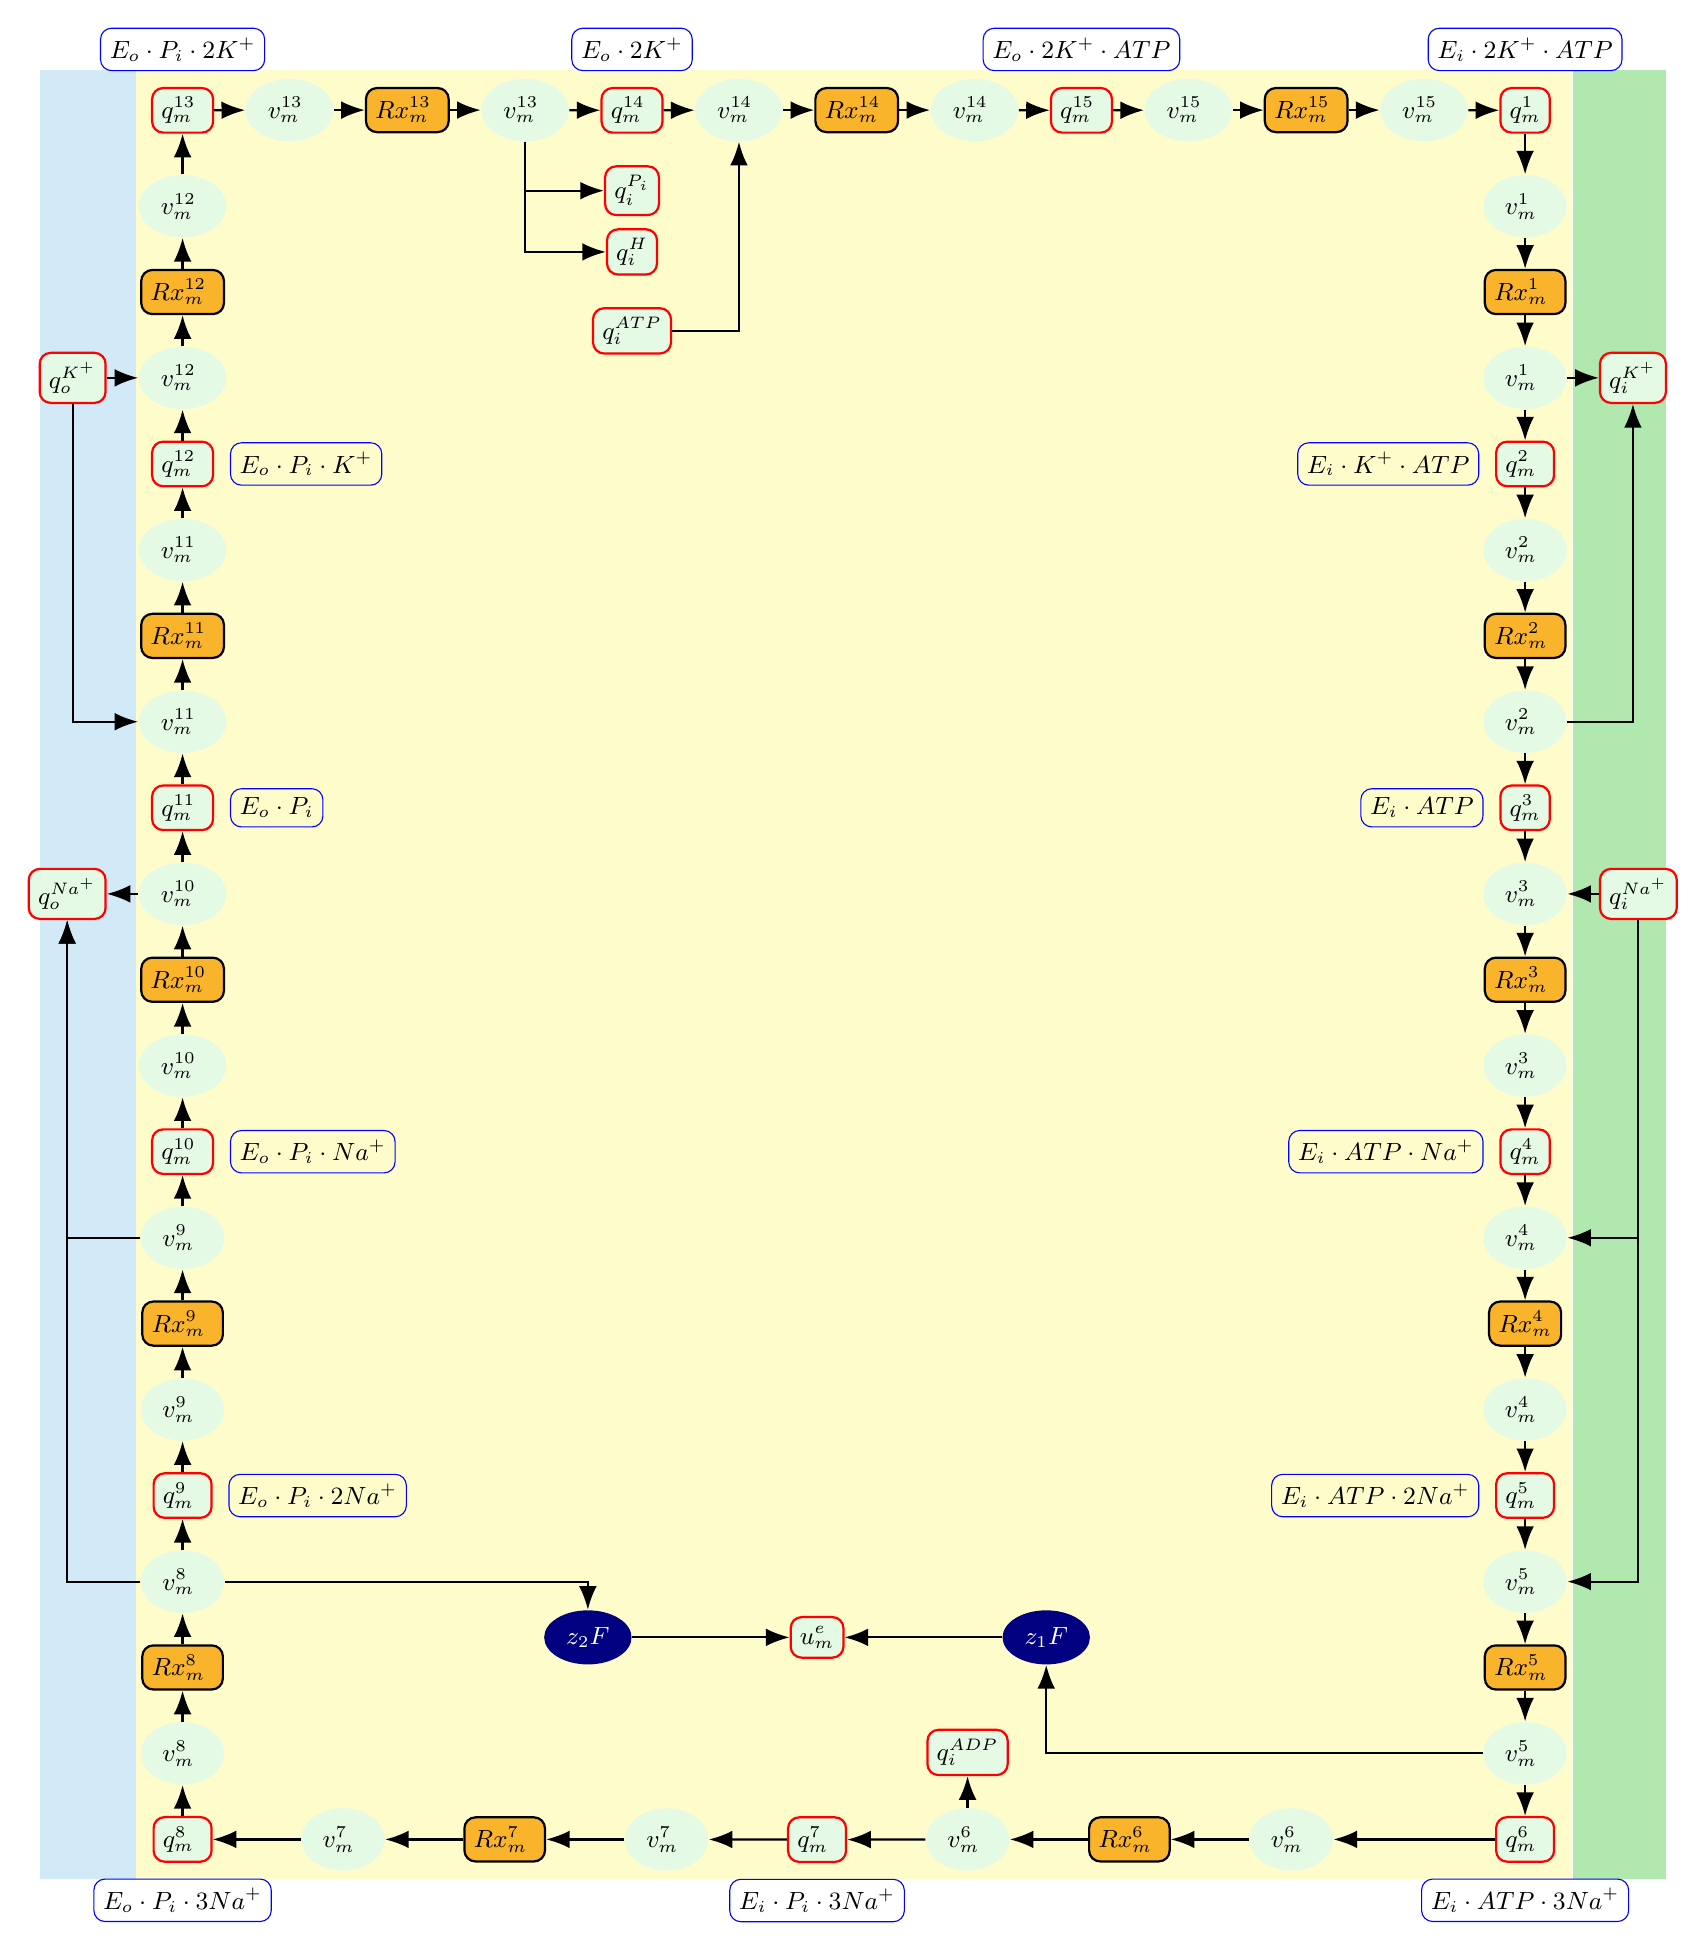
\begin{tikzpicture}[node distance=12mm and 0mm]
% Define the row width (distance between start and end nodes)
\def\rowwidth{60mm}
\def\rowsep{4mm}
\def\colsep{4mm}
\def\colsepp{12mm}
\matrix (top) [matrix of nodes,column sep=\colsep] {
  |[rectred]| $q_m^{13}$ & |[greencycle]| $v_m^{13}$ & |[yellowbox]| $Rx_m^{13}$ & |[greencycle]| $v_m^{13}$ &
  |[rectred]| $q_m^{14}$ & |[greencycle]| $v_m^{14}$ & |[yellowbox]| $Rx_m^{14}$ & |[greencycle]| $v_m^{14}$ &
  |[rectred]| $q_m^{15}$ & |[greencycle]| $v_m^{15}$ & |[yellowbox]| $Rx_m^{15}$ & |[greencycle]| $v_m^{15}$ &
  |[rectred]| $q_m^{1}$\\
};

\foreach \col/\text in {1/$E_o\cdot P_i\cdot 2K^+$,5/$E_o\cdot 2K^+$,
                         9/$E_o\cdot 2K^+\cdot ATP$,13/$E_i\cdot 2K^+\cdot ATP$}{
  \node[rectblue,above=2mm of top-1-\col] (top2-\col) {\text};
}

\matrix (left) [matrix of nodes,row sep=\rowsep, matrix anchor=north, below=\rowsep of top-1-1]  {
|[greencycle]| $v_m^{12}$  \\  |[yellowbox]| $Rx_m^{12}$  \\  |[greencycle]| $v_m^{12}$  \\ |[rectred]| $q_m^{12}$ \\ 
 |[greencycle]| $v_m^{11}$ \\  |[yellowbox]| $Rx_m^{11}$ \\ |[greencycle]| $v_m^{11}$ \\  |[rectred]| $q_m^{11}$  \\ 
 |[greencycle]| $v_m^{10}$  \\  |[yellowbox]| $Rx_m^{10}$  \\  |[greencycle]| $v_m^{10}$ \\   |[rectred]| $q_m^{10}$ \\ 
|[greencycle]| $v_m^{9}$  \\  |[yellowbox]| $Rx_m^{9}$ \\ |[greencycle]| $v_m^{9}$  \\ |[rectred]| $q_m^{9}$ \\ 
 |[greencycle]| $v_m^{8}$ \\ |[yellowbox]| $Rx_m^{8}$  \\ |[greencycle]| $v_m^{8}$  \\ |[rectred]| $q_m^{8}$ \\
};

\foreach \row/\text in {4/$E_o\cdot P_i\cdot K^+$,8/$E_o\cdot P_i$,
                         12/$E_o\cdot P_i\cdot Na^+$,16/$E_o\cdot P_i\cdot 2Na^+$}{
  \node[rectblue,right=2mm of left-\row-1] (left2-\row) {\text};
}
\node[rectblue,below=2mm of  left-20-1] (left2-20)  {$E_o\cdot P_i\cdot 3Na^+$} ;

\matrix (right) [matrix of nodes,row sep=\rowsep, matrix anchor=north, below=\rowsep of top-1-13]  {
 |[greencycle]| $v_m^{1}$  \\ |[yellowbox]| $Rx_m^{1}$ \\  |[greencycle]| $v_m^{1}$ \\  |[rectred]| $q_m^{2}$ \\ 
 |[greencycle]| $v_m^{2}$ \\  |[yellowbox]| $Rx_m^{2}$ \\ |[greencycle]| $v_m^{2}$ \\  |[rectred]| $q_m^{3}$\\ 
  |[greencycle]| $v_m^{3}$ \\  |[yellowbox]| $Rx_m^{3}$ \\  |[greencycle]| $v_m^{3}$ \\ |[rectred]| $q_m^{4}$\\ 
 |[greencycle]| $v_m^{4}$ \\ |[yellowbox]| $Rx_m^{4}$\\  |[greencycle]| $v_m^{4}$ \\  |[rectred]| $q_m^{5}$ \\
 |[greencycle]| $v_m^{5}$ \\  |[yellowbox]| $Rx_m^{5}$ \\ |[greencycle]| $v_m^{5}$ \\  |[rectred]| $q_m^{6}$ \\
};

\foreach \row/\text in {4/$E_i\cdot K^+\cdot ATP$,8/$E_i\cdot ATP$,
                         12/$E_i\cdot ATP\cdot Na^+$,16/$E_i\cdot ATP\cdot 2Na^+$}{
  \node[rectblue,left=2mm of right-\row-1] (right2-\row) {\text};
}

\node[rectblue,below=2mm of  right-20-1] (right2-20)  {$E_i\cdot ATP\cdot 3Na^+$} ;

\matrix (bottom) [matrix of nodes,column sep=10mm, matrix anchor=west, right=10mm of left-20-1]  {
   |[greencycle]| $v_m^{7}$ & |[yellowbox]| $Rx_m^{7}$ & |[greencycle]| $v_m^{7}$ &  |[rectred]| $q_m^{7}$ &
   |[greencycle]| $v_m^{6}$ & |[yellowbox]| $Rx_m^{6}$ & |[greencycle]| $v_m^{6}$ \\
};

\foreach \col/\text in {4/$E_i\cdot P_i\cdot 3Na^+$}{
  \node[rectblue,below=2mm of bottom-1-\col] (bottom2-\col) {\text};
}

\draw[arrow] (left-1-1) -- (top-1-1);
\draw[arrow] (top-1-13) -- (right-1-1);
\draw[arrow] (bottom-1-1) -- (left-20-1);
\draw[arrow] (right-20-1) --(bottom-1-7) ;

\foreach \i in {1,...,12}{
  \pgfmathtruncatemacro{\j}{\i+1} % compute i+1 as integer
  \draw[arrow] (top-1-\i) -- (top-1-\j);
}

\foreach \i in {1,...,6}{
  \pgfmathtruncatemacro{\j}{\i+1} % compute i+1 as integer
  \draw[arrow] (bottom-1-\j) -- (bottom-1-\i);
}
\foreach \i in {1,...,19}{
  \pgfmathtruncatemacro{\j}{\i+1} % compute i+1 as integer
  \draw[arrow] (left-\j-1) -- (left-\i-1);
}
\foreach \i in {1,...,19}{
  \pgfmathtruncatemacro{\j}{\i+1} % compute i+1 as integer
  \draw[arrow] (right-\i-1) -- (right-\j-1);
}

\node[rectred,left=\colsep of left-3-1] (Ko)  {$q_o^{K^+}$} ;
\node[rectred,left=\colsep of left-9-1] (Nao)  {$q_o^{Na^+}$} ;
\node[rectred,right=\colsep of right-3-1] (Ki)  {$q_i^{K^+}$} ;
\node[rectred,right=\colsep of right-9-1] (Nai)   {$q_i^{Na^+}$} ;
\node[rectred,below=\colsep of top-1-5] (Pi)  {$q_i^{P_i}$} ;
\node[rectred,below=\colsepp of top-1-5] (H)  {$q_i^{H}$} ;
\node[rectred,below=\colsep of H] (ATP)  {$q_i^{ATP}$} ;
\node[rectred,above=\colsep of bottom-1-5] (ADP)  {$q_i^{ADP}$} ;
\node[rectred,above=20mm of bottom-1-4] (um)  {$u_m^{e}$} ;
\node[bluecycle,right=20mm of um] (z1)  {\textcolor{white}{$z_1F$}} ;
\node[bluecycle,left=20mm of um] (z2)  {\textcolor{white}{$z_2F$}} ;
\draw[arrow] (z1) -- (um);
\draw[arrow] (z2) -- (um);
\draw[arrow] (right-19-1) -| (z1);
\draw[arrow] (left-17-1) -| (z2);
\draw[arrow] (Ko) -- (left-3-1);
\draw[arrow] (Ko) |- (left-7-1);
\draw[arrow] (left-9-1) -- (Nao);
\draw[arrow] (left-17-1) -| (Nao);
\draw[arrow] (left-13-1) -| (Nao);
\draw[arrow] (right-3-1) -- (Ki);
\draw[arrow] (right-7-1) -| (Ki);
\draw[arrow] (Nai) -- (right-9-1);
\draw[arrow] (Nai) |- (right-13-1) ;
\draw[arrow] (Nai) |- (right-17-1);
\draw[arrow] (bottom-1-5) -- (ADP);
\draw[arrow] (top-1-4) |- (Pi);
\draw[arrow] (top-1-4) |- (H);
\draw[arrow] (ATP) -| (top-1-6);

%=========================
% Background shading
%=========================
\begin{scope}[on background layer]
  \node[fit=(top-1-1)(right-20-1), fill=yellow!20, inner sep=6pt] (fitnode) {};
  \node[fit=(top-1-13)(right-20-1), fill=LimeGreen!90!Gray!40, inner sep=6pt, xshift=12mm] {};
  \node[fit=(top-1-1)(left-20-1), fill=Cerulean!90!Gray!20, inner sep=6pt, xshift=-12mm] {}; 
\end{scope}


\end{tikzpicture}
\end{document}
